
\chapter{引言}
\label{chap:introduction}

\section{研究背景}
文本匹配是自然语言处理中最重要的基础问题之一。许多自然语言处理中的任务例如信息获取,问答系统,机器翻译,对话系统等等,都可以被视为文本匹配问题。根据使用场景的不同,文本匹配可以被分为三类:短文本-短文本匹配,短文本-长文本匹配以及长文本-长文本语义匹配。基于主题模型的语义匹配通常作为经典文本匹配技术的补充,而不是取代传统的文本匹配技术。
\subsection{短文本-短文本匹配}
短文本-短文本的语义匹配在工业界有着非常广泛的应用场景。例如,在网页搜索中,我们需要度量用户查询 (query) 和网页标题 (web page title) 的语义相关性;在知乎等问答网站需要进行相似问题的合并,这时我们需要度量一个问题和其他问题之间的相似度。这些场景都需要短文本-短文本的匹配作为基础。 由于主题模型在短文本上的效果不太理想,在短文本-短文本匹配任务中词向量的应用比主题模型更为普遍。简单的任务可以使用Word2Vec,GLoVE 等模型训练出来的词向量。

比如,在相似问题合并时,我们经常要计算两个问题的相似度,例如“推荐好看的电影”与“经典电影”。通过词向量进行简单处理(例如直接累加),可以得到这两个问题的向量表示。之后可以利用余弦相似度来计算两者的相似度。对于较难的短文本-短文本语义匹配任务,则可以考虑引入有监督信号并利用 Deep Structured Semantic Model(DSSM)\citep{Huang2013LearningDS} 或 Convolutional Latent Semantic Model(CLSM)\citep{Shen2014ALS} 这些更复杂的神经网络模型进行语义相关性的计算。

\subsection{短文本-长文本匹配}
短文本-长文本语义匹配同样在在工业界被广泛运用。例如,在搜索引擎中,我们需要计算一个用户查询(query)和一个网页正文(content)的语义相关度。由于用户查询通常较短,而网页正文较长,因此查询与正文的匹配与上文提到的短文本-短文本不同,通常需要使用短文本-长文本语义匹配,以得到更好的匹配效果。在计算相似度的时候,我们规避对短文本直接进行主题映射,而是根据长文本的主题分布,计算该分布生成短文本的概率,作为它们之间的相似度。

\begin{figure}[!htbp]
    \centering
    
\includegraphics[width=0.40\textwidth]{short_long_query}
    \bicaption{用户查询-广告相似度计算}{Text matching between user and advertise}
    \label{fig:user-ad-match}
\end{figure}

\subsection{长文本-长文本匹配}
通过使用主题模型,我们可以得到两个长文本的主题分布,再通过计算两个多项分布的距离来衡量它们之间的相似度。衡量多项分布的距离可以利用Hellinger Distance\citep{website:Hellinger}和Jensen-Shannon Divergence(JSD)\citep{website:Shannondivergence}

\begin{figure}[!htbp]
  \centering
  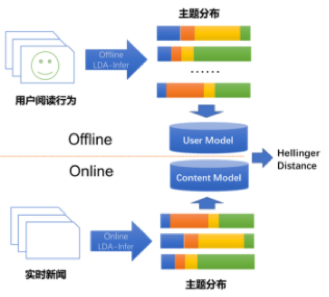
\includegraphics[width=0.4\linewidth]{news_com}
  \caption{新闻个性化推荐}{news recommadation}
  \label{fig:news_recom}
\end{figure}

文本匹配在工业界有着广泛的应用,网页搜索,相似问题合并等等都需要文本匹配作为基础。早期的文本匹配算法往往是对词向量空间如VSM,BM25等的匹配,主要解决基于词汇层面的匹配问题。但是这种算法有很大的局限性:

1. 语言多义性。相同的词语在不同语境下可能拥有不同的含义,如 “苹果” 既可以表示水果,也可以表示科技公司;而不同的词语也可以表达相同的语义,如 “出租车”,“的士”。
2. 语言的组合结构。由相同词语组成的句子由于语序的不同,也可能产生不同的语义。例如 “机器学习” 和 “学习机器”。
3. 匹配的非对称性问题。文本匹配任务并不一定要求语言相似,例如网页搜索中的查询和网页;也不一定要求语义上的相似,例如问答系统。

因此从上世纪 90 年代开始,有人开始尝试将主题模型应用于文本匹配,主题模型可以较好地表示文本的语义信息,从而弥补传统文本匹配算法的不足。但是从效果上看,他们都无法替代基于词汇的匹配方法,只能作为补充。
在世纪初,计算机的计算力和存储量开始爆炸式增长,因此开始有人尝试将深度学习应用于文本匹配算法上并且取得了较好的效果,
目前大部分的深度学习算法都试图利用神经网络理解语义信息,但是现阶段计算机仍然难以理解语义信息,因此基于语义信息的文本匹配算法目前具有天然劣势。

\section{研究意义}
文本匹配是自然语言处理的重要问题,在信息检索、广告计算等领域有着广泛的应用。由于传统的模式匹配方案模式规则难以维护、系统复杂,因此近几年来对文本匹配的研究集中于深度学习,即利用深度网络学习到文本的语义信息进行匹配。但是计算机对语义理解的困难为语义匹配的方案引入了额外的复杂度,算法工程师必须进行巧妙的特征设计以应对不同的业务场景。

近几年来,深度网络极大的增强了强化学习表达能力,使得强化学习建模现实世界问题的能力越来越强。近年来,强化学习已经在文档排序,围棋等等方面发挥越来越重要的作用,而利用强化学习进行文本匹配的相关研究仍然是一片空白。这些领域的规则都远比文本匹配负责,因此利用强化学习学习传统文本匹配中的规则拥有强大的潜力。

\section{本文贡献}
文本匹配是传统的自然语言处理问题,传统的基于模式匹配的方案往往规则复杂,系统难以维护;现在基于深度学习的语义匹配拥有天生的缺陷。而深度强化学习由于其强大的建模能力开始在各个场合发挥越来越重要的作用,因此利用强化学习建模模式匹配,基于大量匹配数据学习匹配规则成为一种可能。本文分析了文本匹配场景下的文本数据特点以及传统文本匹配规则的基础上,提出了基于强化学习的文本匹配算法的解决方案。总体来说本文的贡献在于:

(1)基于 value iteration 算法设计了文本匹配模型

针对于文本匹配场景,本文设计了强化学习中的状态、动作以及奖励函数,并基于 value iteration 算法进行实现求解。通过这一方法,建模了文本匹配中的模式规则,并在 Quora 数据集上将该算法与 MatchPyramid、MatchSrnn 等经典文本匹配算法进行了对比。实验结果表示,基于 value iteration 的文本匹配算法在各个评价准则下均优于其他经典文本匹配算法的效果。

(2)基于 AlphaGo Zero 算法设计了文本匹配模型

基于 value iteration 的文本匹配模型虽然可以建模模式匹配中的规则,但是基于贪心的方法对于语言的组合结构问题有着天生的缺陷。 AlphaGo Zero 算法在设计上降低了局部最优解出现的可能性,因此本文基于 AlphaGo Zero 算法设计了文本匹配模型,并与基于value iteration 文本匹配模型以及其他经典算法进行了对比。实现结果表明,基于 AlphaGo Zero 的文本匹配模型具有显著的优势。

(3)对文本匹配算法进行加速

强化学习虽然拥有强大的建模能力,但是其算法本身的特点导致了它难以加速,且极难利用 GPU 进行并行计算。而 AlphaGo Zero 算法引入的蒙特卡洛树搜索则进一步增长了算法的运行时间。
因此对强化学习算法进行加速以加快训练速度,降低推导延迟是必不可少的。本文基于蒙特卡洛树搜索的特点设计了并行算法,实现了 GPU 和 CPU 协作,大大增加了算法的运行速度

\section{章节安排}
本文共分为六章,每章节的内容组织如下:

第一章为引言部分,主要介绍了基于强化学习的模式文本匹配算法的研究背景以及本文的主要贡献。在本章中,本文首先介绍了文本匹配算法的使用场景,接下来结合现有文本匹配算法的思想,阐述了基于语义的文本匹配算法所具有的缺陷,最后提出了可以利用强化学习建模模式匹配过程,最后介绍了本文的主要贡献。

第二章从两个方面介绍了国内外的研究现状。第一方面是关于文本匹配的研究现状,主要介绍了基于单文档语义以及直接建模匹配的模型;另一方面是强化学习的研究现状,主要介绍了强化学习的基本概念,以及相关算法,为本文之后提出的模型打下基础。

第三章介绍了根据文本匹配问题的特点,设计了强化学习中的 MDP 状态并进行了形式化的描述。根据所提出的 MDP 状态利用 value iteration 算法进行优化,并对实验结果进行分析。

第四章针对于 value iteration 基于贪心的选择方法引入的问题,利用 AlphaGo Zero 框架对 MDP 状态进行优化求解,并根据 AlphaGo Zero 算法的特点对 MDP 状态进行了调整。

第五章针对本文实现的算法进行了高效实现。针对于蒙特卡罗树搜索的特殊场景,设计了 CPU 与 GPU 协作的运行方式,通过流水线的方式对算法进行优化,这个大大加速了算法运行速度,为海量数据场景下的分布式训练带来的可能。

第六章总结了本文的主要贡献与不足。

